\documentclass[11pt]{amsart}
%\pagestyle{empty}
\setlength{\topmargin}{-0.3in} % usually -0.25in
\addtolength{\textheight}{.75in} % usually 1.25in
\addtolength{\oddsidemargin}{-0.5in}
\addtolength{\evensidemargin}{-0.5in}
\addtolength{\textwidth}{1.0in} %\setlength{\parindent}{0pt}

% macros
\usepackage{amssymb,xspace,verbatim}
\usepackage[pdftex]{hyperref}

\usepackage[final]{graphicx}
\newcommand{\regfigure}[3]{\includegraphics[height=#2in,width=#3in]{#1.eps}}

\newtheorem*{thm}{Theorem}
\newtheorem*{lem}{Lemma}

\newcommand{\mtt}{\texttt}
\newcommand{\mtl}[1]{{\texttt{>>#1}}}
\usepackage{alltt}
\usepackage{fancyvrb}

\newcommand{\CC}{{\mathbb{C}}}
\newcommand{\RR}{{\mathbb{R}}}
\newcommand{\ZZ}{{\mathbb{Z}}}
\newcommand{\ZZn}{{\mathbb{Z}}_n}
\newcommand{\NN}{{\mathbb{N}}}

\newcommand{\bu}{\mathbf{u}}
\newcommand{\bv}{\mathbf{v}}

\newcommand{\eps}{\epsilon}
\newcommand{\lam}{\lambda}

\newcommand{\ip}[2]{\mathrm{\left<#1,#2\right>}}
\newcommand{\erf}{\operatorname{erf}}

\newcommand{\Span}{\operatorname{span}}
\newcommand{\rank}{\operatorname{rank}}
\newcommand{\range}{\operatorname{range}}
\newcommand{\Null}{\operatorname{null}}

\renewcommand{\Re}{\operatorname{Re}}

\newcommand{\Matlab}{\textsc{Matlab}\xspace}
\newcommand{\Octave}{\textsc{Octave}\xspace}
\newcommand{\pylab}{\textsc{pylab}\xspace}

\newcommand{\mfile}[1]{
\begin{quote}
\bigskip
\VerbatimInput[frame=single,framesep=3mm,label=\fbox{\normalsize \textsl{\,#1\,}},fontfamily=courier,fontsize=\footnotesize]{../matlab/#1}
\medskip
\end{quote}
}

\DefineVerbatimEnvironment{mVerb}{Verbatim}{numbersep=2mm,
frame=lines,framerule=0.1mm,framesep=2mm,xleftmargin=4mm,fontsize=\footnotesize}

\newcommand{\textbook}{\textsc{Trefethen \& Bau}}

\newcommand{\prob}[1]{\bigskip\noindent\large\textbf{#1.} \normalsize}
\newcommand{\bookprob}[2]{\bigskip\medskip\noindent\large\textbf{Exercise #1 in Lecture #2.} \normalsize}

\newcommand{\ppart}[1]{\textbf{(#1)} }
\newcommand{\epart}[1]{\medskip\noindent\ppart{#1}}


\begin{document}
\scriptsize Math 614 Numerical Linear Algebra (Bueler) \hfill 1 September 2021

\bigskip
\Large\textbf{\centerline{Solutions to Assignment \# 1}}

\medskip
\normalsize
\begin{quote}
\emph{Grading.}  Each part of the multi-part problems (\textbf{P1}, \textbf{P3}, \textbf{P4}) counted as 3 points, and the others (\textbf{P2}, \textbf{Exercise 1.3}) as 5 points.  Total of 31 points.
\end{quote}

\thispagestyle{empty}

\normalsize

\prob{P1}  \ppart{a}  To compute the eigenvalues you can construct the characteristic polynomial $p(\lambda) = \det\left(\lambda I - A\right)$ and find its roots.  I get $p(\lambda) = \lambda^3 - 5 \lambda^2 + 4 \lambda$ so $\lambda = 0, 1, 4$ exactly.

To compute the rank you may do row reduction, and then count the number of nonzero rows.  To compute the determinant you may expand in minors.  Or you can use the above eigenvalues: $\rank(A)=2$ because that is the number of nonzero eigenvalues, and $\det(A)=0$ because that is the product of eigenvalues.

Note $A$ is not invertible.  To invert the lower left two-by-two block $B$ you can use Gauss-Jordan elimination on the augmented matrix $[B|I]$ until it is converted into $[I|B^{-1}]$.  To solve $Av=b$ for the given $b$ you can use row operations to yield an equivalent system with infinitely many solutions:
\begin{align*}
2 x_1 + x_2 + x_3 &= -1 \\
x_2 + 2 x_3 &= -5
\end{align*}
If we let $x_3=s$ then $x_1=2+s/2$, $x_2=-5-2s$, and $x_3=s$ for any $s\in \RR$.

\epart{b} Now check your work in \Matlab:
\begin{mVerb}
>> A = [2 1 1; 4 0 -2; 2 2 3];
>> eig(A)
ans =
   4.00000
  -0.00000
   1.00000
>> rank(A)
ans =  2
>> det(A)
ans = 0
>> inv(A)
warning: matrix singular to machine precision
ans =
       Inf       Inf       Inf  ...
>> format rat,  B = A(2:3,1:2);  inv(B)
ans =
        1/4          0
       -1/4        1/2
>> b = [-1 8 -6]';  A \ b
ans =
      20/21
     -17/21
     -44/21
\end{mVerb}
Note that the last result is for $s=-44/21$; this is one of many correct answers.  (\emph{But why does \Matlab report this one?})

\medskip
\noindent \textbf{Observation}. \Matlab did not do these calculations the way you did them by hand!  And, while \Matlab's methods all generalize to give stable and accurate results for large matrices, the by-hand methods you were taught \emph{do not}.  Thus this course!


\prob{P2}  This code produced Figures 1 and 2:

\mfile{matstats.m}

I did not plot ranks because they are boring.  Of the 80 matrices, in every case $\rank(A)=m$.  Apparently these random matrices are always full rank (invertible).

Figure 1 shows all values of the $\|A\|=$ \texttt{norm(A)}.  These norms vary a little because of the random entries, and they grow slowly with $m$.

\begin{figure}[h]
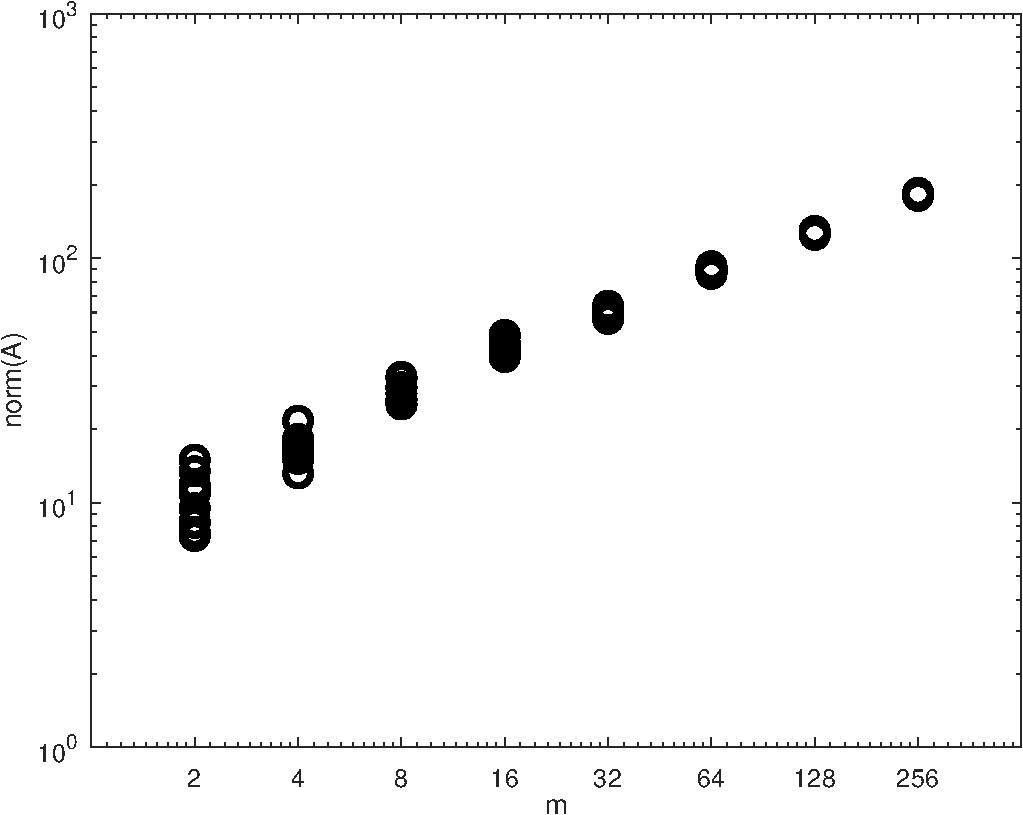
\includegraphics[height=3in,keepaspectratio=true]{a1p2norms}
\caption{For \textbf{P2}:  $\|A\|$ grows slowly with $m$.}
\end{figure}

By contrast, Figure 2 shows that the determinants $|\det(A)| = $\texttt{abs(det(A)))} grow absurdly fast with dimension.  The data for $m=256$ is missing because overflow occurred.  (Our machines can't handle numbers above about $10^{308}$, but there is nothing meaningful in the world that is that large.  There are about $10^{80}$ fundamental particles in the universe!)

\begin{figure}[h]
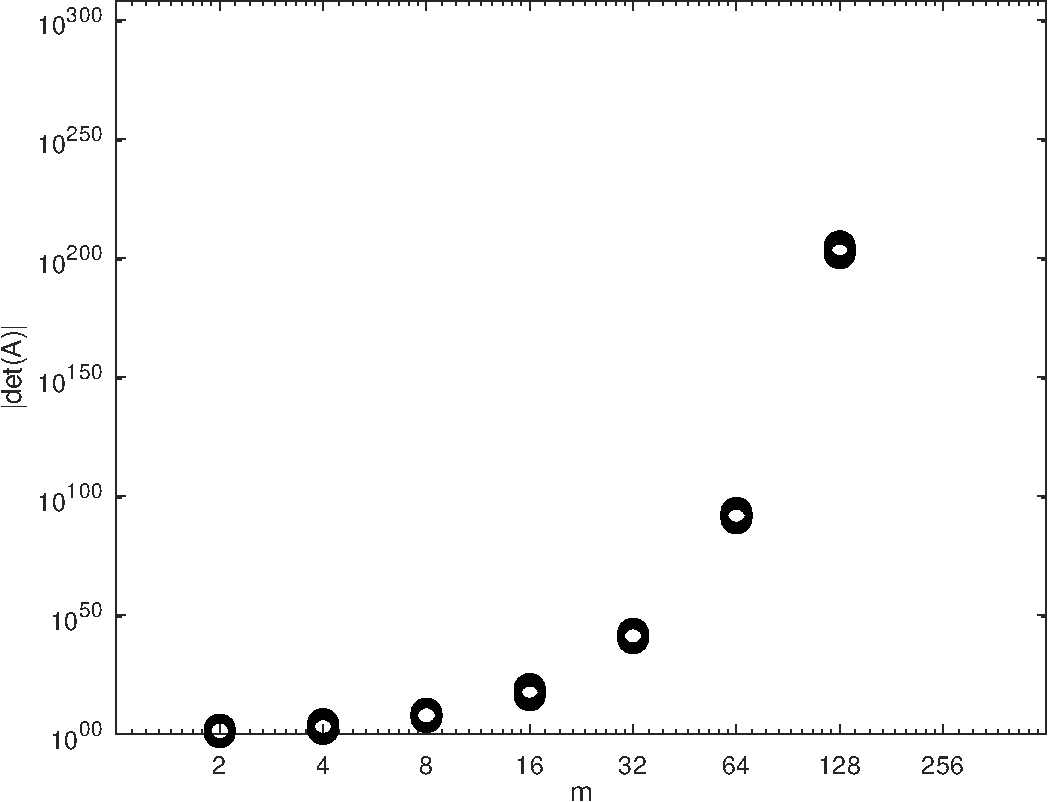
\includegraphics[height=3in,keepaspectratio=true]{a1p2dets}
\caption{For \textbf{P2}:  $|\det(A)|$ grows absurdly fast with $m$.}
\end{figure}


\prob{P3}  \ppart{a}  Let $b=Av$ so $b\in \CC^{m\times 1}$.  The entries of $b$ are computed by this algorithm:
    $$b_j = \sum_{k=1}^n a_{jk} v_k$$
for $j=1,\dots,m$.  The number of multiplications to compute a single entry $b_j$ is thus $n$, and the number of additions is $n-1$.  Therefore the total number of multiplications and additions to compute $Av$ is $mn$ and $m(n-1)$, respectively.

\clearpage
\newpage
\epart{b}  My code looked like this:

\mfile{matvec.m}

\noindent You may check that this works by hand on an example of your choice.  To check that it works the same way as the built-in \texttt{A*v} on random matrices you could do this:
\begin{mVerb}
>> A = randn(4,3);  v = randn(3,1);
>> norm(matvec(A,v) - A*v)
ans = 0
\end{mVerb}
Thus my \texttt{matvec.m} agrees with built-in multiplication.

\epart{c}  Next:

\mfile{matmat.m}

This code does $mkn$ multiplications and $mk(n-1)$ additions for a total of $mk(2n-1)$ operations.  Finally, I compared against built-in multiplication on random matrices:
\begin{mVerb}
>> A = randn(3,4);  B = randn(4,3);
>> norm(matmat(A,B) - A*B)
ans = 0
\end{mVerb}

\medskip
Though it is \emph{not} requested in the Assignment, it is interesting to compare speeds:
\begin{mVerb}
>> A = rand(51,87);  B = randn(87,64);
>> tic, C=A*B; toc, tic, C=matmat(A,B); toc
Elapsed time is 0.000834942 seconds.
Elapsed time is 3.68026 seconds.
>> A = rand(251,187);  B = randn(187,164);
>> tic, C=A*B; toc, tic, C=matmat(A,B); toc
Elapsed time is 0.00689316 seconds.
Elapsed time is 99.039 seconds.
\end{mVerb}
The speed of my version is disastrous, $10^4$ times slower!  This \texttt{matmat.m} code will be much faster in \Matlab than in \Octave, and yet faster in Julia, but still not near the built-in.  Why do you think the built-ins are so much faster?


\prob{P4}  \ppart{a}  The fundamental idea of this exercise is that
\begin{itemize}
\item operations that act on ROWs are implemented by LEFT multiplication
\item operations on COLUMNs are RIGHT multiplications.
\end{itemize}

So here is what I did.  I used \Matlab by starting with a $4\times 4$ matrix with distinct integer entries.  (Distinct entries makes it easier to follow through the steps.)  For each operation I simply tacked on a row operation (on the left) or a column operation (on the right) as appropriate.  I checked that each had the intended effect.  Run the following code to see what I did.

\mfile{manipulations.m}

The result is the product
    $$L_7 L_5 L_4 L_1 B R_2 R_3 R_6.$$

\epart{b}  If $A = L_7 L_5 L_4 L_1$ and $C = R_2 R_3 R_6$ then the result of part \textbf{(a)} is the product $ABC$.  Displaying these matrices allows us to check our work:
    $$A = \begin{bmatrix}
         0 &        1 &        0 &        0 \\
         1 &       -1 &        0 &        0 \\
         0 &       -1 &        0 &        1
    \end{bmatrix},
    \qquad
    C = \begin{bmatrix}
         1 &        0 &        0 &        0 \\
         0 &        0 &        1 &        1 \\
         0 &        0 &        0 &        0 \\
         0 &        1 &        0 &        0
    \end{bmatrix}$$


\bookprob{1.3}{1}  \emph{There are other ways to do it, but I think this was intended.  Note that triangular matrices are invertible if and only if all of their diagonal entries are nonzero.}
\medskip

\noindent If $R\in\CC^{m\times m}$ is a nonsingular upper-triangular matrix then $R^{-1}$ is upper-triangular.

\newcommand{\trefmatrixthree}[3]{\left[\begin{array}{c|c|c|c} & & & \\ #1 & #2 & \dots & #3 \\ & & & \end{array}\right]}

\begin{proof}  Let $B=R^{-1}$, the unknown inverse.  (\emph{We know it exists, but we are trying to prove it is triangular.})  We write $I=BR$ and think of this product as the columns of $R$ acting to give linear combinations of the (unknown) columns of $B$ to produce the known columns $e_j$ of the identity:
$$\trefmatrixthree{e_1}{e_2}{e_m} = \trefmatrixthree{b_1}{b_2}{b_m} \left[\begin{array}{c|c|c|c} r_{11} & r_{12} & \dots & r_{1m} \\  & r_{22} & \dots & r_{2m} \\ & & \ddots & \vdots \\  & & & r_{mm}\end{array}\right]$$
As equations for columns this says:
\begin{align*}
e_1 &= r_{11} b_1 \\
e_2 &= r_{12} b_1 + r_{22} b_2 \\
e_3 &= r_{13} b_1 + r_{23} b_2 + r_{33} b_3 \\
&\vdots \\
e_m &= r_{1m} b_1 + r_{2m} b_2 + r_{3m} b_3 + \dots + r_{mm} b_m
\end{align*}
Since we know $R$ is invertible it follows that these equations have unique solutions.  That is, these equations determine the columns $b_j$.

The first two equations (i.e.~equality in the first two columns) say
    $$\begin{bmatrix} 1 \\ 0 \\ \vdots \\ 0 \end{bmatrix} = \begin{bmatrix} r_{11} b_{11} \\ r_{11} b_{21} \\ \vdots \\ r_{11} b_{m1} \end{bmatrix}, \qquad \qquad \begin{bmatrix} 0 \\ 1 \\ \vdots \\ 0 \end{bmatrix} = \begin{bmatrix} r_{12} b_{11} + r_{22} b_{12} \\  r_{12} b_{21} + r_{22} b_{22} \\ \vdots \\ r_{12} b_{m1} + r_{22} b_{m2} \end{bmatrix}.$$
The first says $r_{11} b_{11} = 1$, so $b_{11} = 1/r_{11}$, and it says $b_{21}=b_{31}= \dots =b_{m1}=0$.  Now that we know $b_{i1}$ for $i=1,2,\dots,m$, we can use the second column equation to solve for $b_{i2}$.  For $i=1,2$ we have $b_{12} = - (r_{12} b_{11}) / r_{22}$ and $b_{22} = (1 - r_{12} b_{21}) / r_{22} = (1 - 0) / r_{22} = 1/r_{22}$.  However, for $i=3,\dots,m$ we have $b_{i2}=- (r_{12} b_{i1}) / r_{22} = 0 / r_{22} = 0$.

Continuing in this way we get formulas for $b_{ij}$, and in particular we get $b_{ij}=0$ if $i>j$.  (That is, we can actually write down the entries of $R^{-1}$.)  Thus $B=R^{-1}$ is upper triangular.\end{proof}

\end{document}
